%%
%%  Example paper
%%
%%

%%%%%%%%%%%%%%%%%% Usenix style %%%%%%%%%%%%%%%%%%%%%%%%%%%%%%%%%
\documentclass[10pt,twocolumn,a4paper]{article}
\usepackage{styles/usenix-style}

\author{Jakob Schmid}

%%%%%%%%%%%%%%%%%% Document %%%%%%%%%%%%%%%%%%%%%%%%%%%%%%%%%%%%%%%%%%%
% TODO: Change draft to final before submitting final version.
\usepackage[draft]{styles/ka-style}
\usepackage{cite,xspace,ifthen,graphicx,listings,url}

\usepackage[
   pdfauthor={Author},
   pdftitle={A Paper Template},
   pdfsubject={Paper Template},
   pdfkeywords={Papers, Templates}
]{hyperref}

\begin{document}

\title{Unikernel Linux (UKL)}

\newcommand{\todo}[1]{{\texttt{[#1]}}}
\newcommand{\code}[1]{{\tt \small{#1}}}
\newcommand{\refsec}[1]{{§ \ref{#1}}}

\maketitle
%\draftfooter

\begin{abstract}
  This report discusses Unikernel Linux (UKL), an approach to introduce a
  unikernel target into the Linux kernel.
  The specialized demand of cloud services has recently given rise
  to a resurgence of library operating systems in the form of unikernels.
  The authors of the UKL paper want to show that the Linux kernel can be
  modified to include the benefits of unikernels, while maintaining the
  ecosystem of applications and maintainers of Linux.
\end{abstract}

\section{Introduction}\label{sec:introduction}
  Modern cloud services are often highly specialised, to the point of a microservice, 
  where an applications is split up into a collection of loosely coupled services,
  that communicate through lightweight protocols and each only fullfill a single purpose.
  These services share a few key demands. They need to be able to communicate 
  efficiently with each other. Since they need to communicate with other services,
  they are exposed to the internet to some degree and thus should be as secure as possible.
  Due to the single purpose nature of the microservices they often execute as a single process.
  Lastly the image the service is executed with and the memory usage should be as small as possible.
  The services are often executed in a virtual machine on rented hardware, so lower requirements
  in memory and storage can improve the profitability of a service.
  These demands have caused a resurgence of research exploring the concept of 
  a library operating system (libOS) and the emergence of unikernels. 

  In a libOS a target application is linked with a set of
  libraries that provide all the services a regular OS would usually provide.
  The resulting executable can then be deployed directly to hardware.
  In 2013 the term \textit{unikernel} was first introduced for libOSs
  for cloud services and deployment to virtual hardware \cite{madhavapeddy13}.

  Since then multiple unikernels have been created. Some are written from scratch like
  ClickOS \cite{martins2014} and Unikraft \cite{kuenzer21}.
  Others borrow code from an existing OS like Drawbridge \cite{porter11} 
  that uses code from Windows.

  UKL uses the Linux kernel as a base but tries to keep the changes minimal
  so that UKL can be maintained with the (general purpose) Linux kernel.
  

\section{Background}\label{sec:background}
  \subsection{General-purpose monolithic operating systems}
    In a general-purpose monolithic operating system, such as Linux and Windows,
    the operating system (OS) defines an interface to use the physical resources
    of the system. 
    This interface hides details about the physical resources behind
    high-level abstractions like processes, files, addresss spaces 
    and interprocess communication.
    Applications running on the system use this interface and its abstractions
    to utilize the physical resources of the system.
    The implementation of the abstractions must be general to allow the execution 
    of very different applications.
    The OS also ensures that different applications can execute concurrently, 
    without interfering with each other. 
    Virtual address spaces are used to allow for simultanious usage of physical memory.
    Access to other resources, such as files and network communication, is controlled
    by the OS.
    This protection requires that applications must not be able
    to modify or replace the implementation of the abstractions supplied by the OS.

  \subsection{Library operating systems}\label{sec:libOS}
    One of the problems of the fixed abstractions for system resources in general-purpose OSs
    is that it denies applications the advantage of domain-specific optimizations.
    For example in 1994 Cao et al. \cite{cao94} showed that application-controlled file caching
    can reduce application running time by 45\%.

    In the mid 1990s the libOS was proposed as a different OS architecture
    where the application can control the hardware abstractions, instead of the OS \cite{engler95}.
    In a libOS the hardware resources are not controlled and protected by a kernel.
    Instead a set of application-level libraries implement the mechanisms to drive hardware,
    communicate over the network and all other functionality a general-purpose 
    operating system would provide for an application.
    Further a set of policies are used to enforce access control and isolation in the
    application layer \cite{madhavapeddy13-2}.
    
    The libOS architecture allows applications to access hardware resources directly
    thus eliminating the need for repeated privilege transitions to move data
    between kernel and user space.
    In addition applications can now choose a library to drive the hardware that is
    taylored to the needs of that specific application, thus improving performance.
    This architecture also makes the performance more predictable.
    In a monolithic OS the kernel might schedule a different process after a
    context switch or do signal handling before handing control back to the application.

    Compiling an application with only the libraries the application requires
    can significantly reduce the amount of code involved.
    This reduction in code can not only lead to a reduction in image size, 
    but can also decrease the chance of the code containing a 
    security vulnerability \cite{madhavapeddy13}.

    The libOS architecture has two major disadvantages:   
    One, it is hard to achieve strong resource isolation because not all
    usage of hardware resources has to go through one abstraction supplied by
    a kernel like in a monolithic OS.
    Two, device drivers have to be rewritten to work as a library rather than
    for example a kernel module.
    This implementation effort has caused problems with hardware compatability
    for libOS projects and thus mostly limited their relevance to the
    research domain \cite{madhavapeddy13}.

  \subsection{Unikernels}
    OS virtualisation can overcome both of the major disadvantages of libOSs
    mentioned in \refsec{sec:libOS}.
    The lack of resource isolation between applications can be avoided by
    dedicating a seperate virtual machine (VM) to each application.
    This delegates resource isolation from the OS level to the hypervisor.
    The hypervisor offers a much simpler, less fine grained interface than
    a conventional OS, consisting of virtual CPUs and memory pages, 
    rather than the process-oriented approach in conventional OSs \cite{madhavapeddy13-2}.
    Dedicating a seperate VM to each application also leaves more room
    to specialize the VM to its particular purpose.
    The problem of hardware compatability of libOSs can also be overcome
    with virtualization. The libOS only has to implement drivers for
    the virtual hardware devices offered by the hypervisor.
    The hypervisor is then responsibel for driving the ever changing physical
    hardware.

    Madhavapeddy et al. introduced the term unikernel in a paper 
    published in 2013 \cite{madhavapeddy13}.
    Here unikernels are described as an approach to deploy cloud services
    using specialised single-purpose libOS VMs running directly 
    on the hypervisor \cite{madhavapeddy13}.
    
    Deploying a service using a unikernel can offer significant
    performance advantages. 
    Memcached running on a unikernel TCP/IP stack
    demonstrated a 200\% throughput improvement compared to Linux \cite{schatzberg16},
    unikernels deployed within a microVM have shown six to ten times shorter
    boot times over containers \cite{koller17} and a micropython unikernel reached an image
    size of 1MB while requireing 8MB of memory to run \cite{manco17}.

    Further the security of an appliance can also be improved by using a unikernel.
    About 70\% of vulnerabilities in Windows that Microsoft assigns a CVE each year
    are memory safety issues \cite{msrc-19-07}.
    Unikernels written in high level programming languages with a strong type system 
    can use high level language features for memory management to negate a large
    portion of these vulnerabilities \cite{madhavapeddy13, lankes19}.
    MirageOS \cite{madhavapeddy13}, a unikernel written in OCaml, can be sealed \cite{hunt07} at runtime,
    thus preventing any code not present at compile time from being executed.
    MirageOS further implements compile-time address space randomization to defend against
    return-oriented programming attacks and save on runtime complexity.
    This is justified by the fact that for unikernels reconfiguring the appliance 
    means recompiling it, potentially for every deployment \cite{madhavapeddy13}.

    Another aspect of unikernel security is that the chance for a common exploit is lower.
    An exploit found in the linux kernel can potentially affect all machines running Linux
    due to them sharing a vast majority of their code.
    Each unikernel however is specialized to suit the needs of only one application thus
    sharing less code with other appliances using the same unikernel.
    The smaller amount of shared code decreases the probability of an exploit being applicable
    to many unikernel appliances.

    

    


\begin{figure}[htbp]
  \centering
  \fbox{\parbox{.8\columnwidth}{
      Here you can include a sample figure.  Use something like
      \begin{center}
        \code{$\backslash$includegraphics[scale=.8]\{template\}}
      \end{center}
      to include an encapsulated postscript figure.  The \emph{scale}
      argument can be used for scaling the picture, although it
      may scale the font incorrectly.
    }}
  \caption{Sample Figure}
  \label{fig:sample}
\end{figure}


\lstset{language=C, basicstyle=\ttfamily,
        string=[b]', showspaces=false, showtabs=false,
        caption={A sample code snippet}, captionpos=b}
\begin{lstlisting}
/* code snippet  */
while (!sleep)
	sleep++;
\end{lstlisting}

\begin{figure}[hbt]
\centering
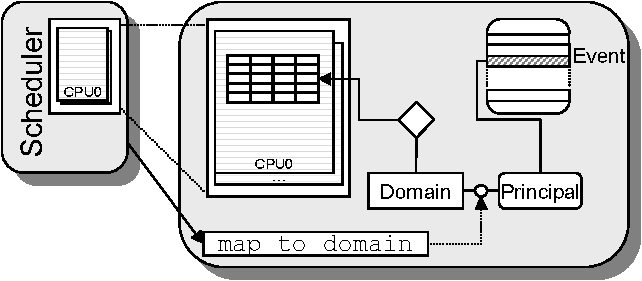
\includegraphics[scale=.7,clip]{fig/template}
\caption{Sample figure automatically from Windows prn.\label{plot:fig}}
\end{figure}

\section{Related Work}\label{sec:relwork} 

Works \cite{xen03virtualization} and \cite{pratt2005xaa} are relevant but
different.

\section{Approach}

\section{Conclusion}\label{sec:conclusion}

\bibliographystyle{plain}
\bibliography{template}
%\footnotesize
\end{document}
